\section{Overview}

Judas and TinyDAS are created with the intention of processing DAS data as efficiently as possible, and subsequentially detect anomalies within said data. 

In the figure below, we see how Judas and TinyDAS can be utilized to both process and train or analyse DAS data.

\begin{figure}[!h]
    \centering
    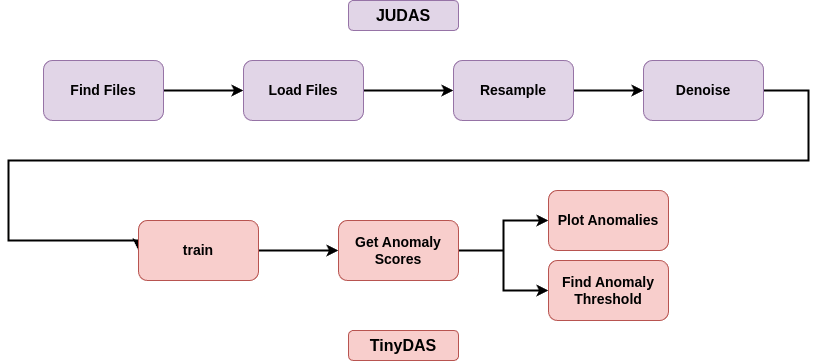
\includegraphics[scale=.5]{figures/api_overview.png}
    \caption{Judas and TinyDAS combined methodflow}
    \label{fig:judasnet_overview}
\end{figure}